\documentclass{beamer}

\usepackage[utf8]{inputenc}
\usepackage[spanish]{babel}
\usepackage{amsmath}
\usepackage{amssymb}
\usepackage{tikz}
\usetikzlibrary{arrows,calc,positioning}
\usetheme{Goddard}
\hypersetup{colorlinks,allcolors=.,urlcolor=magenta}

\title{Investigación de Operaciones II}
\subtitle{Unidad 1: Análisis de Redes}
\author{Ricardo Jesús Largaespada Fernández}
\institute{Ingeniería de Sistemas, DACTIC, UNI}
\date{25 de Marzo, 2025}

\begin{document}

% ---------------------------------------------------------------
% TÍTULO Y AGENDA
% ---------------------------------------------------------------
\frame{\titlepage}

\begin{frame}{Agenda}
    \tableofcontents
\end{frame}

% ---------------------------------------------------------------
% SESIÓN 5
% ---------------------------------------------------------------
\section{Sesión 8}

% ---------------------------------------------------------------
% FRAME: Sesión 5 - Introducción
% ---------------------------------------------------------------
\begin{frame}{Sesión 8}
\textbf{Tema:}
\begin{enumerate}
    \item Método de la Ruta Crítica.
\end{enumerate}

\textbf{Objetivo:}
\begin{itemize}
    \item El estudiante encontrará la duración de un proyecto usando el método de la ruta crítica.
\end{itemize}
\end{frame}

%-----------------------------------------------
\subsection{¿Qué son CPM y PERT?}
\begin{frame}
\frametitle{¿Qué son CPM y PERT?}

\begin{itemize}
    \item Métodos basados en redes para planificar, programar y controlar proyectos.
    \item \textbf{CPM (Critical Path Method)}: Se centra en actividades con duraciones determinísticas.
    \item \textbf{PERT (Program Evaluation and Review Technique)}: Maneja actividades con duraciones probabilísticas.
    \item Ambos métodos permiten identificar la secuencia crítica de actividades y estimar el tiempo total de ejecución.
\end{itemize}

\end{frame}

%-----------------------------------------------
\subsection{Objetivo de CPM y PERT}
\begin{frame}
\frametitle{Objetivo de CPM y PERT}

\begin{itemize}
    \item Proporcionar herramientas analíticas para la \textbf{programación y control} de actividades.
    \item Determinar la \textbf{secuencia lógica} y los \textbf{tiempos} de cada actividad.
    \item Localizar la \textbf{ruta crítica} (o rutas críticas) que condiciona el tiempo mínimo de finalización del proyecto.
\end{itemize}

\end{frame}

%-----------------------------------------------
\subsection{Pasos de CPM/PERT}
\begin{frame}
\frametitle{Pasos de CPM/PERT}

\begin{center}
    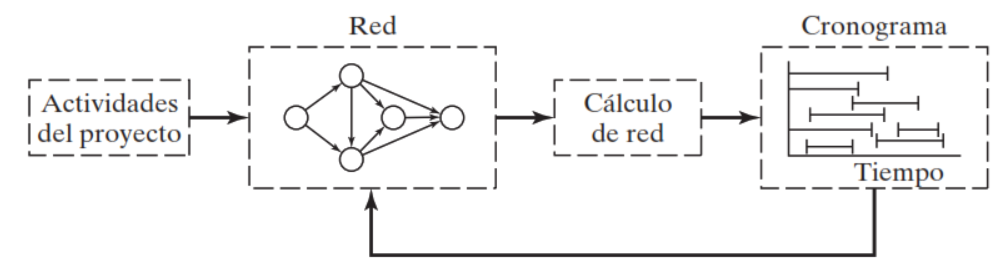
\includegraphics[scale=0.4]{images/fases_proyecto.png}
\end{center}
\begin{enumerate}
    \item \textbf{Definir las actividades} del proyecto (descomposición en tareas).
    \item \textbf{Establecer las relaciones de precedencia} y estimar los tiempos requeridos para cada actividad.
    \item \textbf{Modelar la red} de actividades mediante nodos y arcos, siguiendo las reglas de construcción.
    \item \textbf{Calcular el cronograma}: determinación de fechas tempranas, fechas tardías, holguras y ruta(s) crítica(s).
\end{enumerate}

\end{frame}

%-----------------------------------------------
\begin{frame}
\frametitle{Retroalimentación en la ejecución}

\begin{itemize}
    \item Las actividades pueden presentar \textbf{desviaciones} respecto al plan original.
    \item El cronograma debe \textbf{actualizarse} según la ejecución real.
    \item Se establece un \textbf{bucle de retroalimentación} para \textbf{recalcular y controlar} el proyecto de forma dinámica.
\end{itemize}

\end{frame}

%-----------------------------------------------
\begin{frame}
\frametitle{Diferencias clave entre CPM y PERT}

\begin{itemize}
    \item \textbf{CPM}:
    \begin{itemize}
        \item Duraciones determinísticas (basadas en promedios o experiencia histórica).
        \item Enfoque en la \textbf{ruta crítica} para optimizar recursos y costos.
    \end{itemize}
    \item \textbf{PERT}:
    \begin{itemize}
        \item Duraciones probabilísticas (tres estimaciones: optimista, más probable y pesimista).
        \item Permite \textbf{calcular la probabilidad} de acabar en un tiempo dado.
    \end{itemize}
\end{itemize}

\end{frame}

%-----------------------------------------------
\subsection{Representación en red}
\begin{frame}
\frametitle{Representación en red}

\begin{itemize}
    \item Una \textbf{actividad} se representa por un \textbf{arco} (flecha) que une dos nodos.
    \item Un \textbf{nodo} representa un \textbf{evento} (inicio o final) y determina la precedencia entre actividades.
    \item También se puede usar la notación de \textbf{Actividad en Nodo (AoN)}, según el estándar del PMBOK.
\end{itemize}

\end{frame}

%-----------------------------------------------
\subsubsection{Reglas de construcción de la red (Método AoA)}
\begin{frame}
\frametitle{Reglas de construcción de la red (Método AoA)}

\begin{itemize}
    \item \textbf{Regla 1}: Cada actividad está representada por un solo \textbf{arco}.
    \item \textbf{Regla 2}: Cada actividad debe tener nodos terminales \textbf{distintos} (evitar que dos actividades diferentes compartan origen y destino idénticos).
    \item \textbf{Regla 3}: Verificar siempre precedencia:
        \begin{itemize}
            \item (a) ¿Qué actividades preceden a la actual?
            \item (b) ¿Qué actividades siguen a la actual?
            \item (c) ¿Qué actividades son concurrentes?
        \end{itemize}
\end{itemize}

\end{frame}

%-----------------------------------------------
\begin{frame}
\frametitle{Actividad ficticia}

\begin{itemize}
    \item Representa \textbf{concurrencia} o dependencia sin consumo de tiempo ni recursos.
    \item Se dibuja con una \textbf{flecha discontinua}, entre dos nodos.
    \item Ayuda a resolver problemas de precedencia y evitar duplicidades de nodos.
\end{itemize}

\end{frame}

%-----------------------------------------------
\begin{frame}
\frametitle{Ejemplo con actividad ficticia}

\textbf{Problema}: Las actividades A y B no pueden tener los mismos nodos de inicio y fin.

\textbf{Solución}: Usar un nodo intermedio y una \textbf{actividad ficticia} que respete las reglas de construcción.

\begin{center}
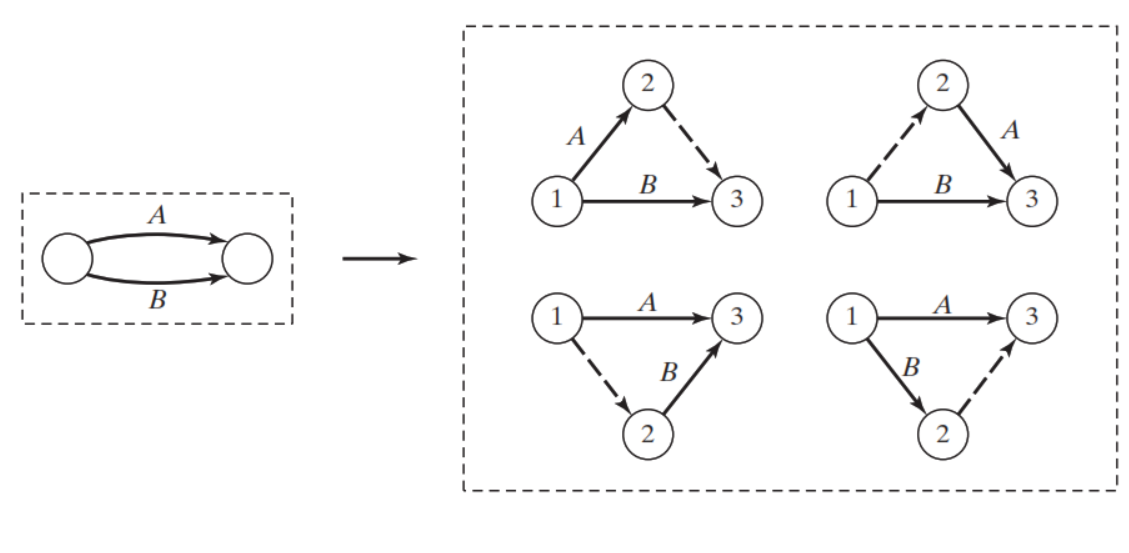
\includegraphics[scale=0.3]{images/actividad_ficticia.png}
\end{center}

\end{frame}

%-----------------------------------------------
\begin{frame}
\frametitle{Fases de CPM-PERT}

\begin{enumerate}
    \item \textbf{Definir} todas las actividades y estimar sus tiempos.
    \item \textbf{Construir} la red (identificar secuencias y dependencias).
    \item \textbf{Calcular} los tiempos en la red (tempranos, tardíos, holguras, ruta crítica).
    \item \textbf{Generar} el cronograma y diagramas de Gantt (opcional).
    \item \textbf{Realizar la retroalimentación} en la ejecución: ajustar según eventos reales.
\end{enumerate}

\end{frame}

%-----------------------------------------------
\begin{frame}
\frametitle{Uso de actividades ficticias}

\begin{itemize}
    \item Se utilizan para \textbf{garantizar la precedencia} correcta de ciertas actividades.
    \item Permiten representar \textbf{restricciones múltiples} y concurrencia.
    \item No tienen duración (0) ni consumo de recursos, pero son esenciales para la coherencia de la red.
\end{itemize}

\end{frame}

%-----------------------------------------------
\begin{frame}
\frametitle{Ejemplo de precedencia}

\begin{enumerate}
    \item Actividad C inicia cuando A y B han finalizado.
    \item Actividad E inicia sólo después de que B finalice.
    \item Si no se maneja correctamente, podría imponerse una falsa dependencia de A sobre E.
\end{enumerate}

\end{frame}

%-----------------------------------------------
\begin{frame}
\frametitle{Representación}

\begin{itemize}
    \item Al dibujar A y B hacia un mismo nodo, \textbf{E} termina dependiendo también de \textbf{A}.
    \item Esto viola la precedencia real: se introducen dependencias inexistentes.
\end{itemize}

% Ejemplo de diagrama incorrecto
\begin{center}
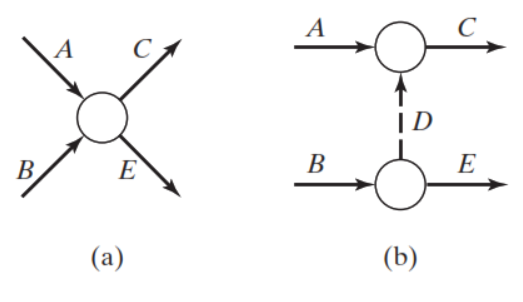
\includegraphics[scale=0.4]{images/actividad_concurrente.png}
\end{center}
\vspace{-1cm}
\begin{itemize}
    \item Se introduce una \textbf{actividad ficticia} (D) para separar la dependencia de C (que requiere A y B) de la de E (que sólo requiere B).
    \item Así, C depende de A \textbf{y} B, mientras E depende únicamente de B.
\end{itemize}

\end{frame}

\begin{frame}{Ejemplo: Construcción de una Red}
    Un editor firmó un contrato con un autor para publicar un libro de texto. El autor somete a consideración una copia impresa de un archivo de computadora del manuscrito. Las actividades (simplificadas) asociadas con la producción del libro de texto se resumen en la siguiente tabla.
    \begin{center}
        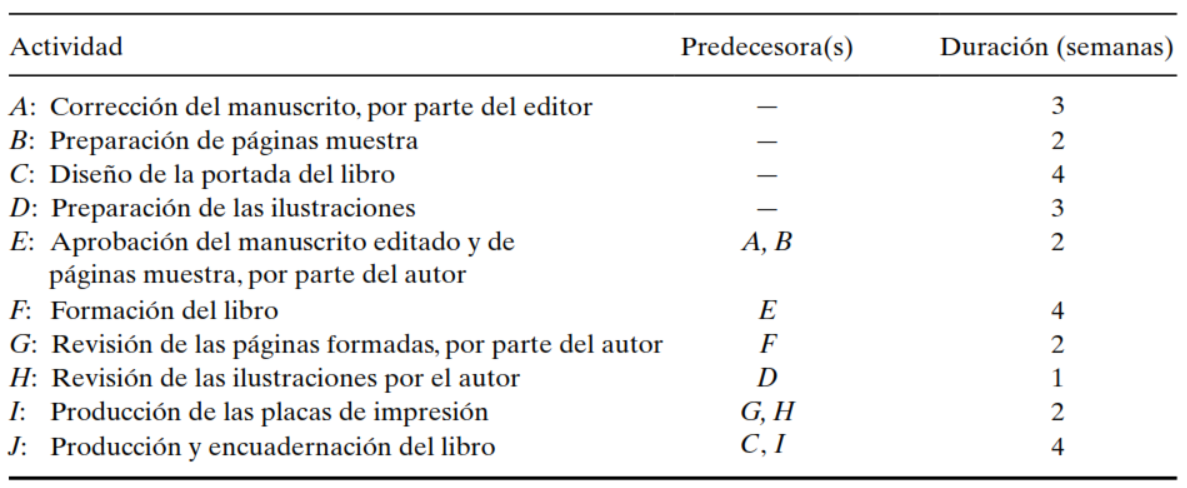
\includegraphics[scale=0.3]{images/08_ejemplo_2.png}
    \end{center}
\end{frame}

\begin{frame}{Solución: Construcción de una Red}
   \begin{center}
       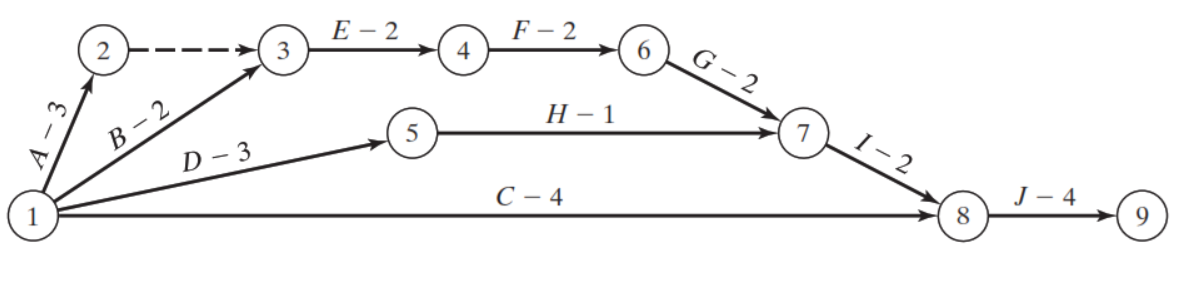
\includegraphics[width=\linewidth]{images/08_sol_ejemplo_2.png}
   \end{center} 
\end{frame}

\subsection{Cálculos del método de la ruta crítica (CPM)}
\begin{frame}{Cálculos del método de la ruta crítica (CPM)}
    El resultado final en el CPM es un cronograma para el proyecto. 
    Para lograr este objetivo se realizan cálculos especiales para obtener la siguiente información:
    
    \begin{enumerate}
        \item \textbf{Duración total} necesaria para completar el proyecto.
        \item \textbf{Clasificación} de las actividades del proyecto como \textit{críticas} o \textit{no críticas}.
    \end{enumerate}
\end{frame}

\subsubsection{Clasificación de actividades}
\begin{frame}{Actividades críticas y no críticas}
    Una actividad es \textbf{crítica} si sus tiempos de inicio y terminación están predeterminados (fijos). 
    
    Una actividad es \textbf{no crítica} si puede ser programada en un espacio de tiempo mayor que su duración, 
    lo que permite tiempos de inicio y terminación flexibles (dentro de los límites). 
    
    Una demora en el tiempo de inicio de una actividad crítica definitivamente retrasa la terminación del proyecto, 
    en tanto que una demora en una actividad no crítica quizá no afecte la fecha de terminación del proyecto.
\end{frame}

\begin{frame}{Definición de evento en la ruta crítica}
    \subsubsection{Eventos en CPM}
    Para realizar los cálculos necesarios, definimos un \textbf{evento} como un punto en el tiempo en el cual se completan las actividades y se inician las subsiguientes. En función de la red, un evento corresponde a un nodo. Sean:

    \[
    \square_j = \text{Tiempo de ocurrencia más temprano del evento } j
    \]
    \[
    \Delta_j = \text{Tiempo de ocurrencia más tardío del evento } j
    \]
    \[
    D_{ij} = \text{Duración de la actividad } (i,j)
    \]

\end{frame}

\begin{frame}{Cálculos de tiempos en CPM}
    \subsubsection{Tiempos y pasos en CPM}
    Todos los tiempos de ocurrencia se miden a partir del inicio del proyecto. El lapso $(\square_j, \Delta_j)$ define el periodo de tiempo durante el cual se programa la actividad $(i,j)$ de duración $D_{ij}$. 

    Si la actividad $(i,j)$ es \textbf{crítica}, entonces:
    \[
    D_{ij} = \Delta_j - \square_j
    \]
    De lo contrario:
    \[
    D_{ij} < \Delta_j - \square_i
    \]
    para la actividad \textbf{no crítica} $(i,j)$. 
    
    Los cálculos de la ruta crítica implican dos pasos: 
    \begin{itemize}
        \item El \textbf{paso adelantado} determina los tiempos de ocurrencia \textit{más tempranos} de los eventos.
        \item El \textbf{paso retrasado} calcula sus tiempos de ocurrencia \textit{más tardíos}.
    \end{itemize}
\end{frame}

\subsubsection{Paso adelantado}
\begin{frame}{Paso Adelantado}
    \begin{center}
        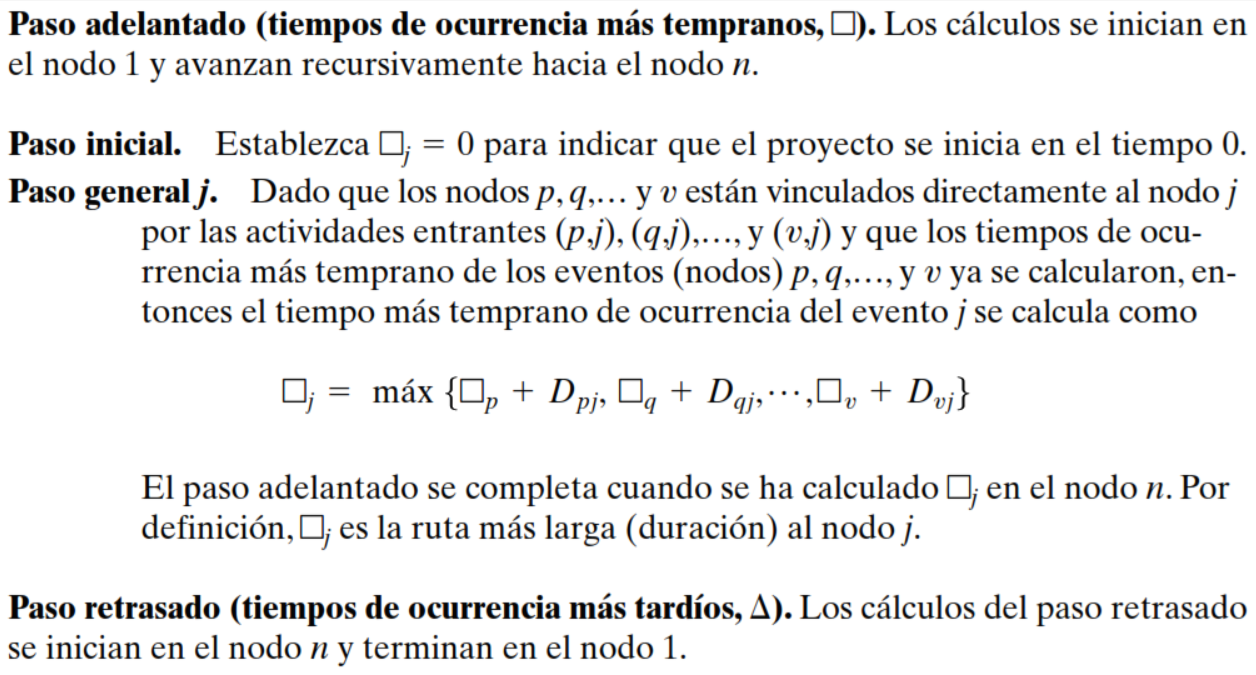
\includegraphics[width=\linewidth]{images/08_paso_adelantado.png}
    \end{center}
\end{frame}

\subsubsection{Paso retrasado}
\begin{frame}{Paso Retrasado}
    \begin{center}
        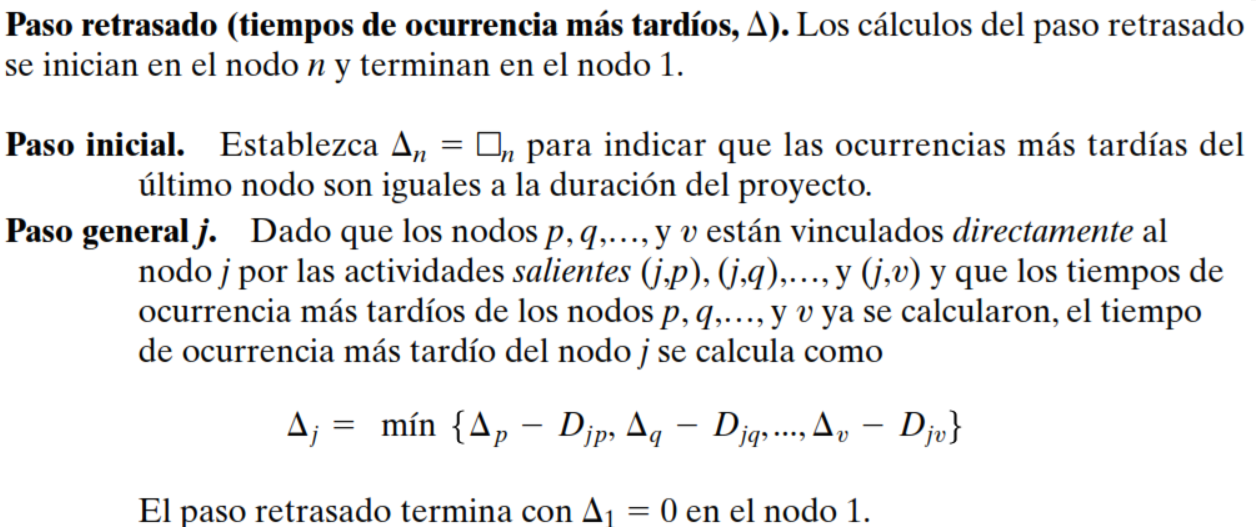
\includegraphics[width=\linewidth]{images/08_paso_retrasado.png}
    \end{center}
\end{frame}

\subsubsection{Determinación de la ruta crítica}
\begin{frame}{Determinación de la Ruta Crítica}
    Con base en los cálculos anteriores, una actividad \((i,j)\) será crítica si satisface tres condiciones.
    \begin{enumerate}
\item \(\Delta_i=\square_i\)
\item \(\Delta_i=\square_j\)
\item \(\Delta_j-\square_i= D_{ij}\)
\end{enumerate}
Las tres condiciones establecen que los tiempos de ocurrencia más tempranos y más tardíos de los nodos finales $i$ y $j$ son iguales y que la duración $D_{ij}$ encaja ``perfectamente'' en el espacio de tiempo especificado. Una condición que no satisface las tres condiciones es \textit{no crítica}.
Por definición, las actividades críticas de una red constituyen la ruta más larga que abarca el proyecto desde el inicio hasta la terminación.
\end{frame}
\end{document}
